\documentclass[12pt,letterpaper]{article}

%% Language and font encodings
\usepackage[english]{babel}
\usepackage[utf8x]{inputenc}
\usepackage[T1]{fontenc}
\usepackage{tikz}
\usetikzlibrary{calc,patterns,decorations.pathmorphing,decorations.markings}
\usepackage{float}
\usepackage{caption}
\usepackage{subcaption}
\usepackage{setspace}
\usepackage{ragged2e}

%% Sets page size and margins
\usepackage[top=3cm,bottom=2cm,left=3cm,right=3cm,marginparwidth=1.75cm]{geometry}
\geometry{letterpaper}
%\usepackage[justification=centering]{caption}
\usepackage{caption}
%% Useful packages
\usepackage{amsmath}
\usepackage{graphicx}
\usepackage{titlesec}
\usepackage{array}
\titlelabel{\thetitle.\quad}
\usepackage{graphicx}
\usepackage[colorinlistoftodos]{todonotes}
\usepackage[colorlinks=true, allcolors=blue]{hyperref}
\usepackage{listings}
\usepackage[autostyle]{csquotes}
\usepackage{hyperref}
\usepackage[hyphenbreaks]{breakurl}


% TITLE PAGE
\title{URA-2019}
% \author{Loic James Azzalini}
% \email{jazzalin@uwaterloo.ca}

%DOCUMENT
\begin{document}

    % Titlepage
    \newpage
    \pdfbookmark[0]{Main Title}{maintitle}
    \begin{titlepage}
        \centering
        \vspace {1.5cm}
        \Large{\textbf{Rotary Double Inverted Pendulum Experiment}} \\ [0.75cm]
        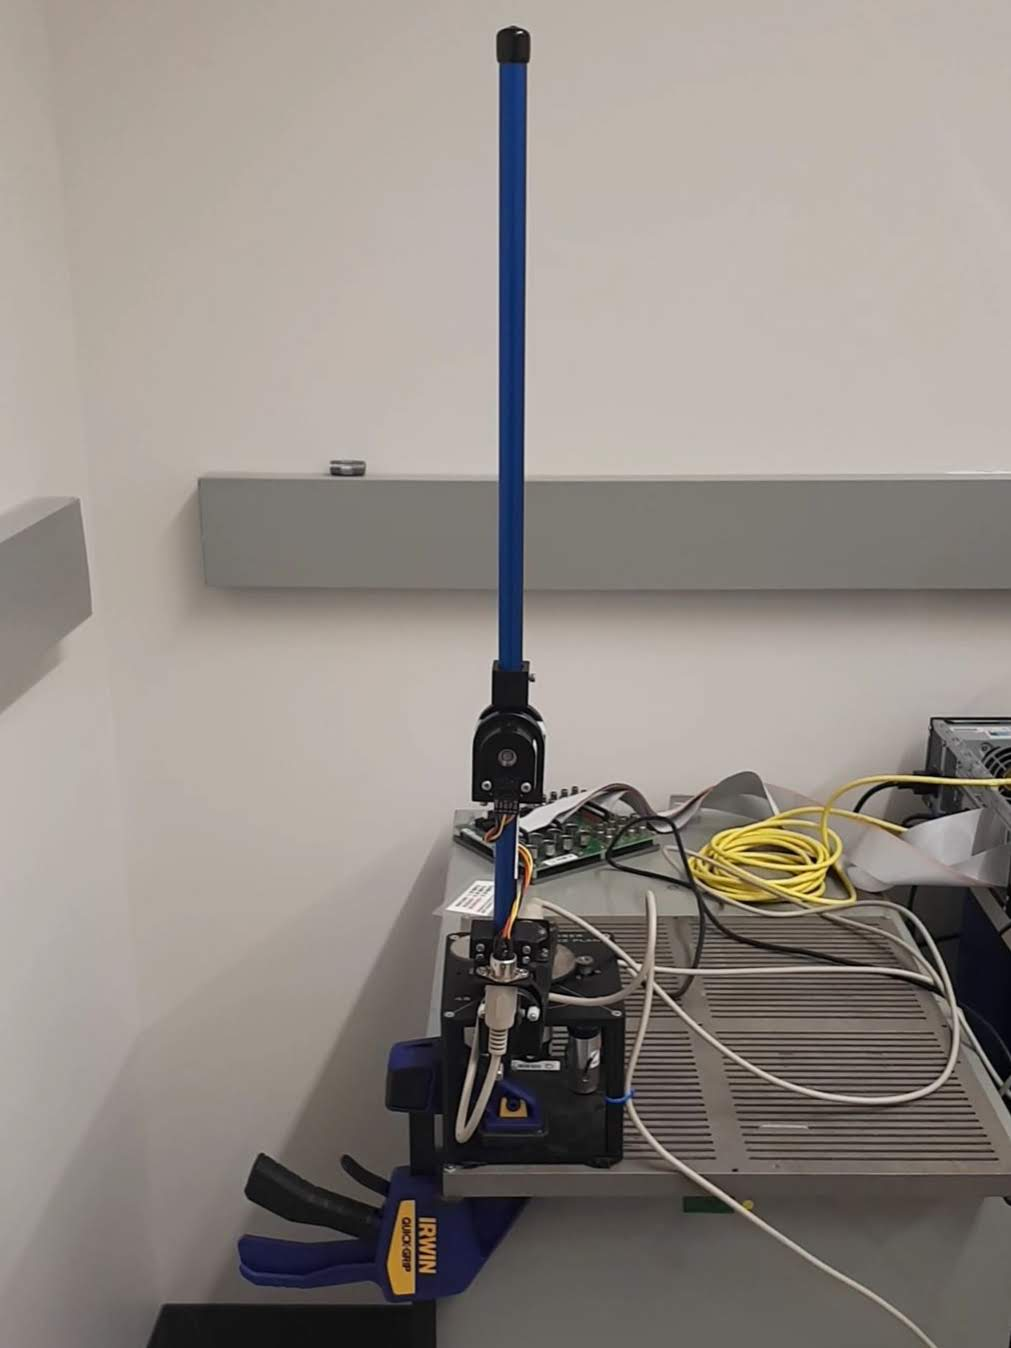
\includegraphics[scale=0.35]{img/front.jpg}
        \vspace {1.00cm}

        \normalsize{Department of Electrical and Computer Engineering \\
        University of Waterloo \\
        Waterloo, Canada} \\ [0.75 cm]
        \today
    \end{titlepage}
\newpage

\setcounter{page}{1}
\pagenumbering{arabic}
\setlength{\parindent}{0pt}
% \onehalfspacing

%INTRODUCTION
\section{Introduction}

A rotary double inverted pendulum was setup in the hope of supporting research in the application of virtual holonomic constraints (VHC) to dynamic systems in the future. The QUANSER apparatus was setup in the lab and connected to a Windows workstation running MATLAB/Simulink and Quarc. A basic balancing controller was successfully implemented and tested on the system.

\section{Setup}

The main changes brought to the setup are summarized below:

\begin{itemize}
    \item Gathered the pendulum apparatus and set it up with the workstation in E7-5411
    \item Used the Q8-USB device instead of the older (now deprecated) Q8 board
    \item Checked that all three encoders correctly reported tick counts
    \item Acquired a base plate from the ECE department to anchor the pendulum to the workbench (a clamp was used in the meantime)
    \item Checked that a basic controller would run on the system
\end{itemize}


\subsection{Hardware setup}

The hardware was setup according to the wiring diagram provided by QUANSER.

\begin{figure}[H]
\centering
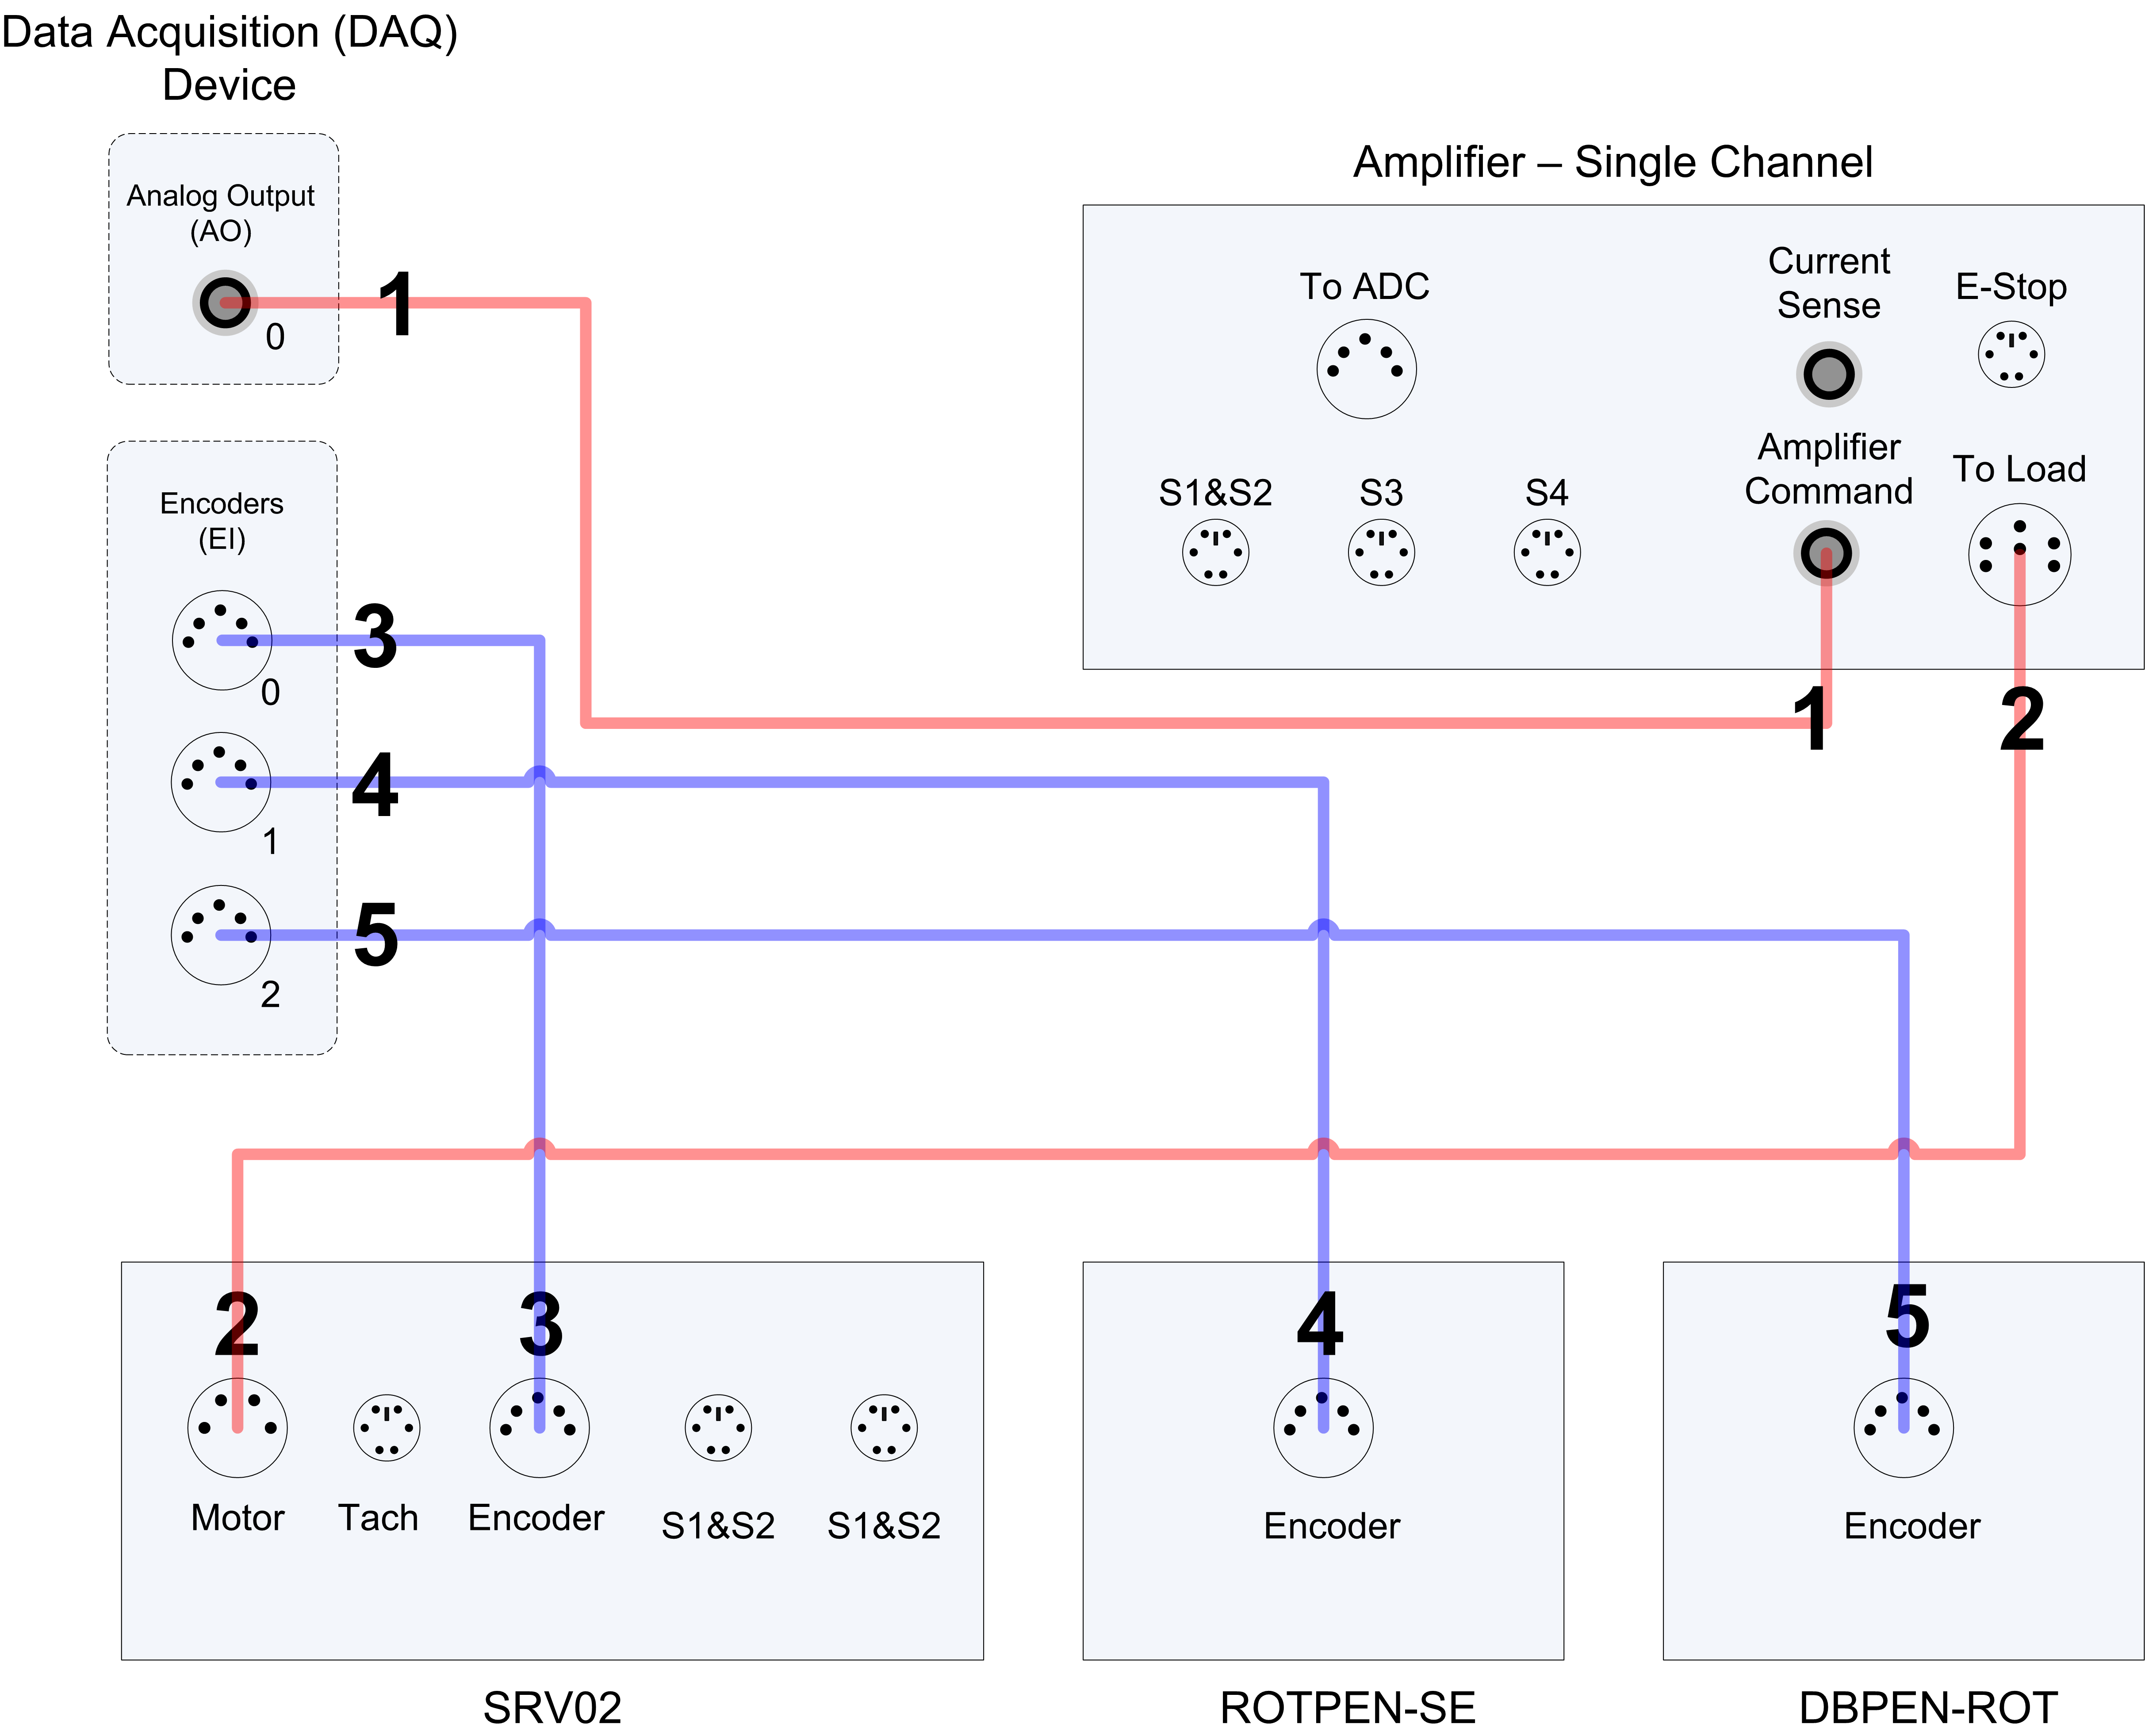
\includegraphics[width=0.7\linewidth]{img/wiring.png}
\caption[Simulation results]{Wiring between the pendulum base, data acquisition module (DAQ) and amplifier}
\label{fig:wiring}
\end{figure}

The Q8-USB DAQ was found to work better than the now deprecated Q8 board (which needs to be directly connected to the computer's motherboard). The Q8-USB board connects to one of the computer's port via standard USB 2.0 A-male to B-male. It connects to the amplifier via RCA male and to the different encoders on the pendulum via 5-pin stereo-DIN cables.


\begin{figure}[H]
\centering
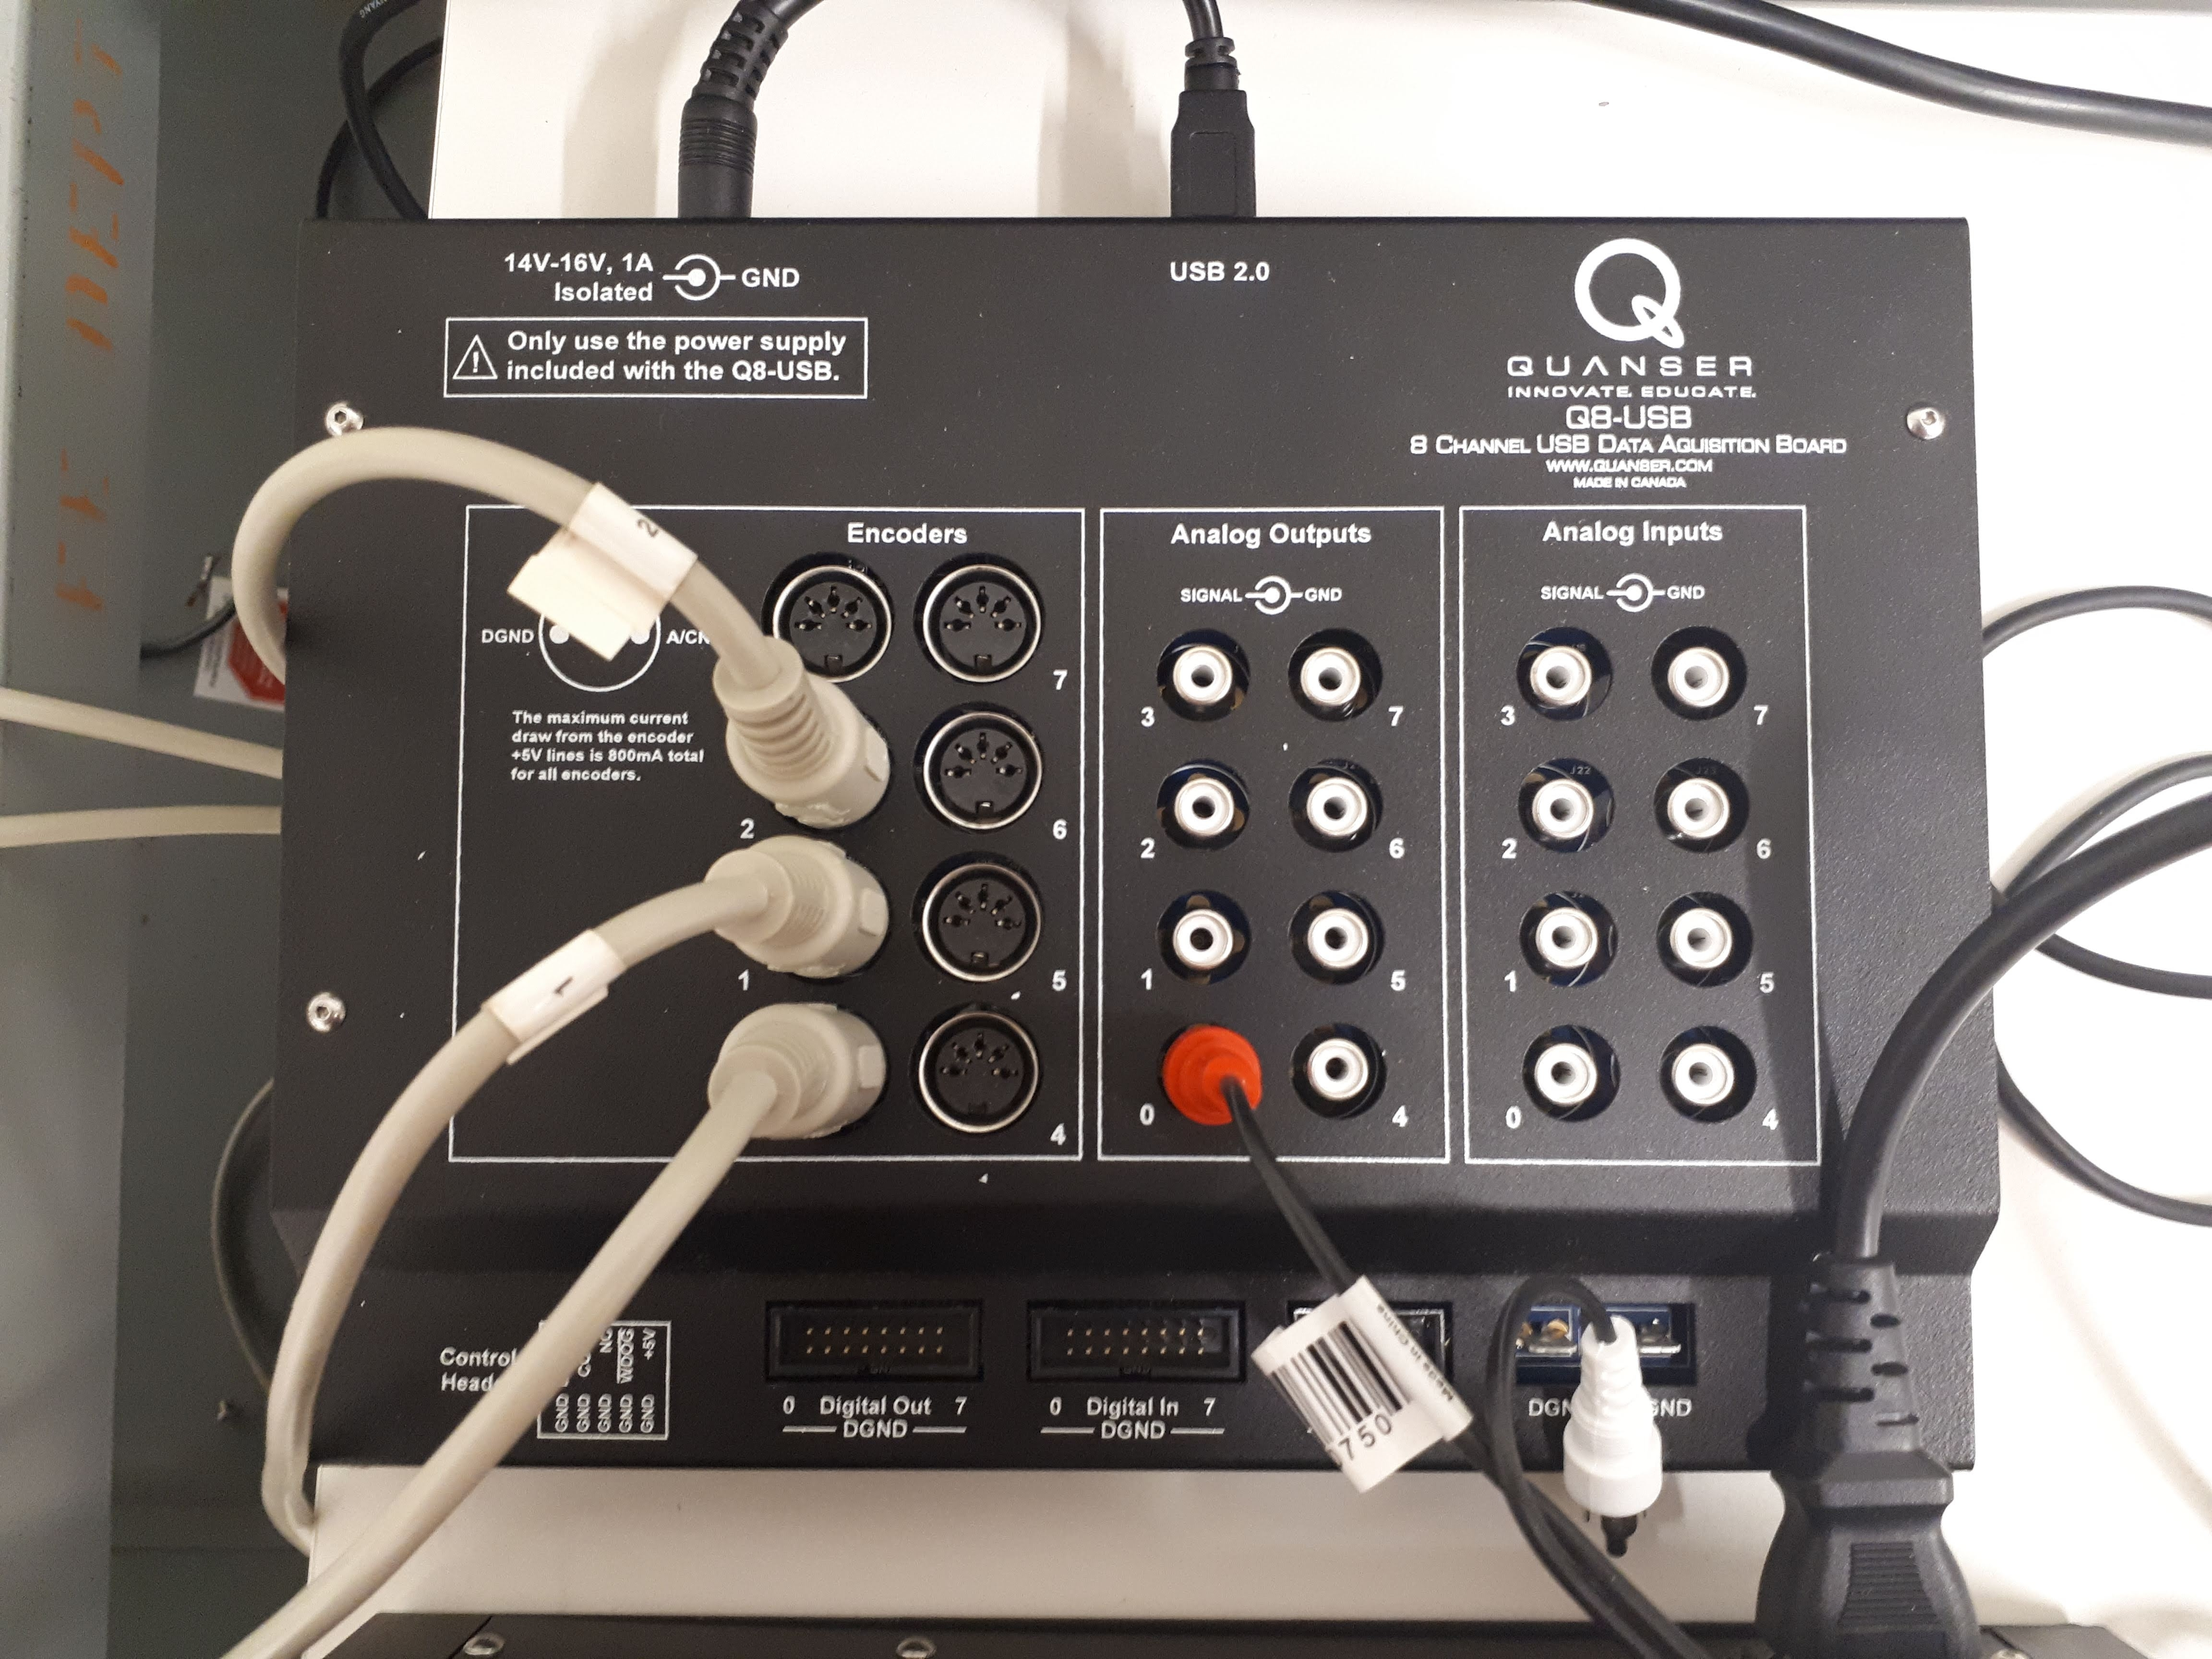
\includegraphics[scale=0.07]{img/daq.jpg}
\caption[Simulation results]{The Q8-USB data acquisition board (DAQ)}
\label{fig:daq}
\end{figure}

The amplifier (VoltPAQ-X1) powers the DC motor attached to the pendulum base (SRV02) via a 4-pin DIN to 6-pin DIN cable. Note that the amplifier gain is set to 1x, which needs to match with the code settings input later on.

\begin{figure}[H]
\centering
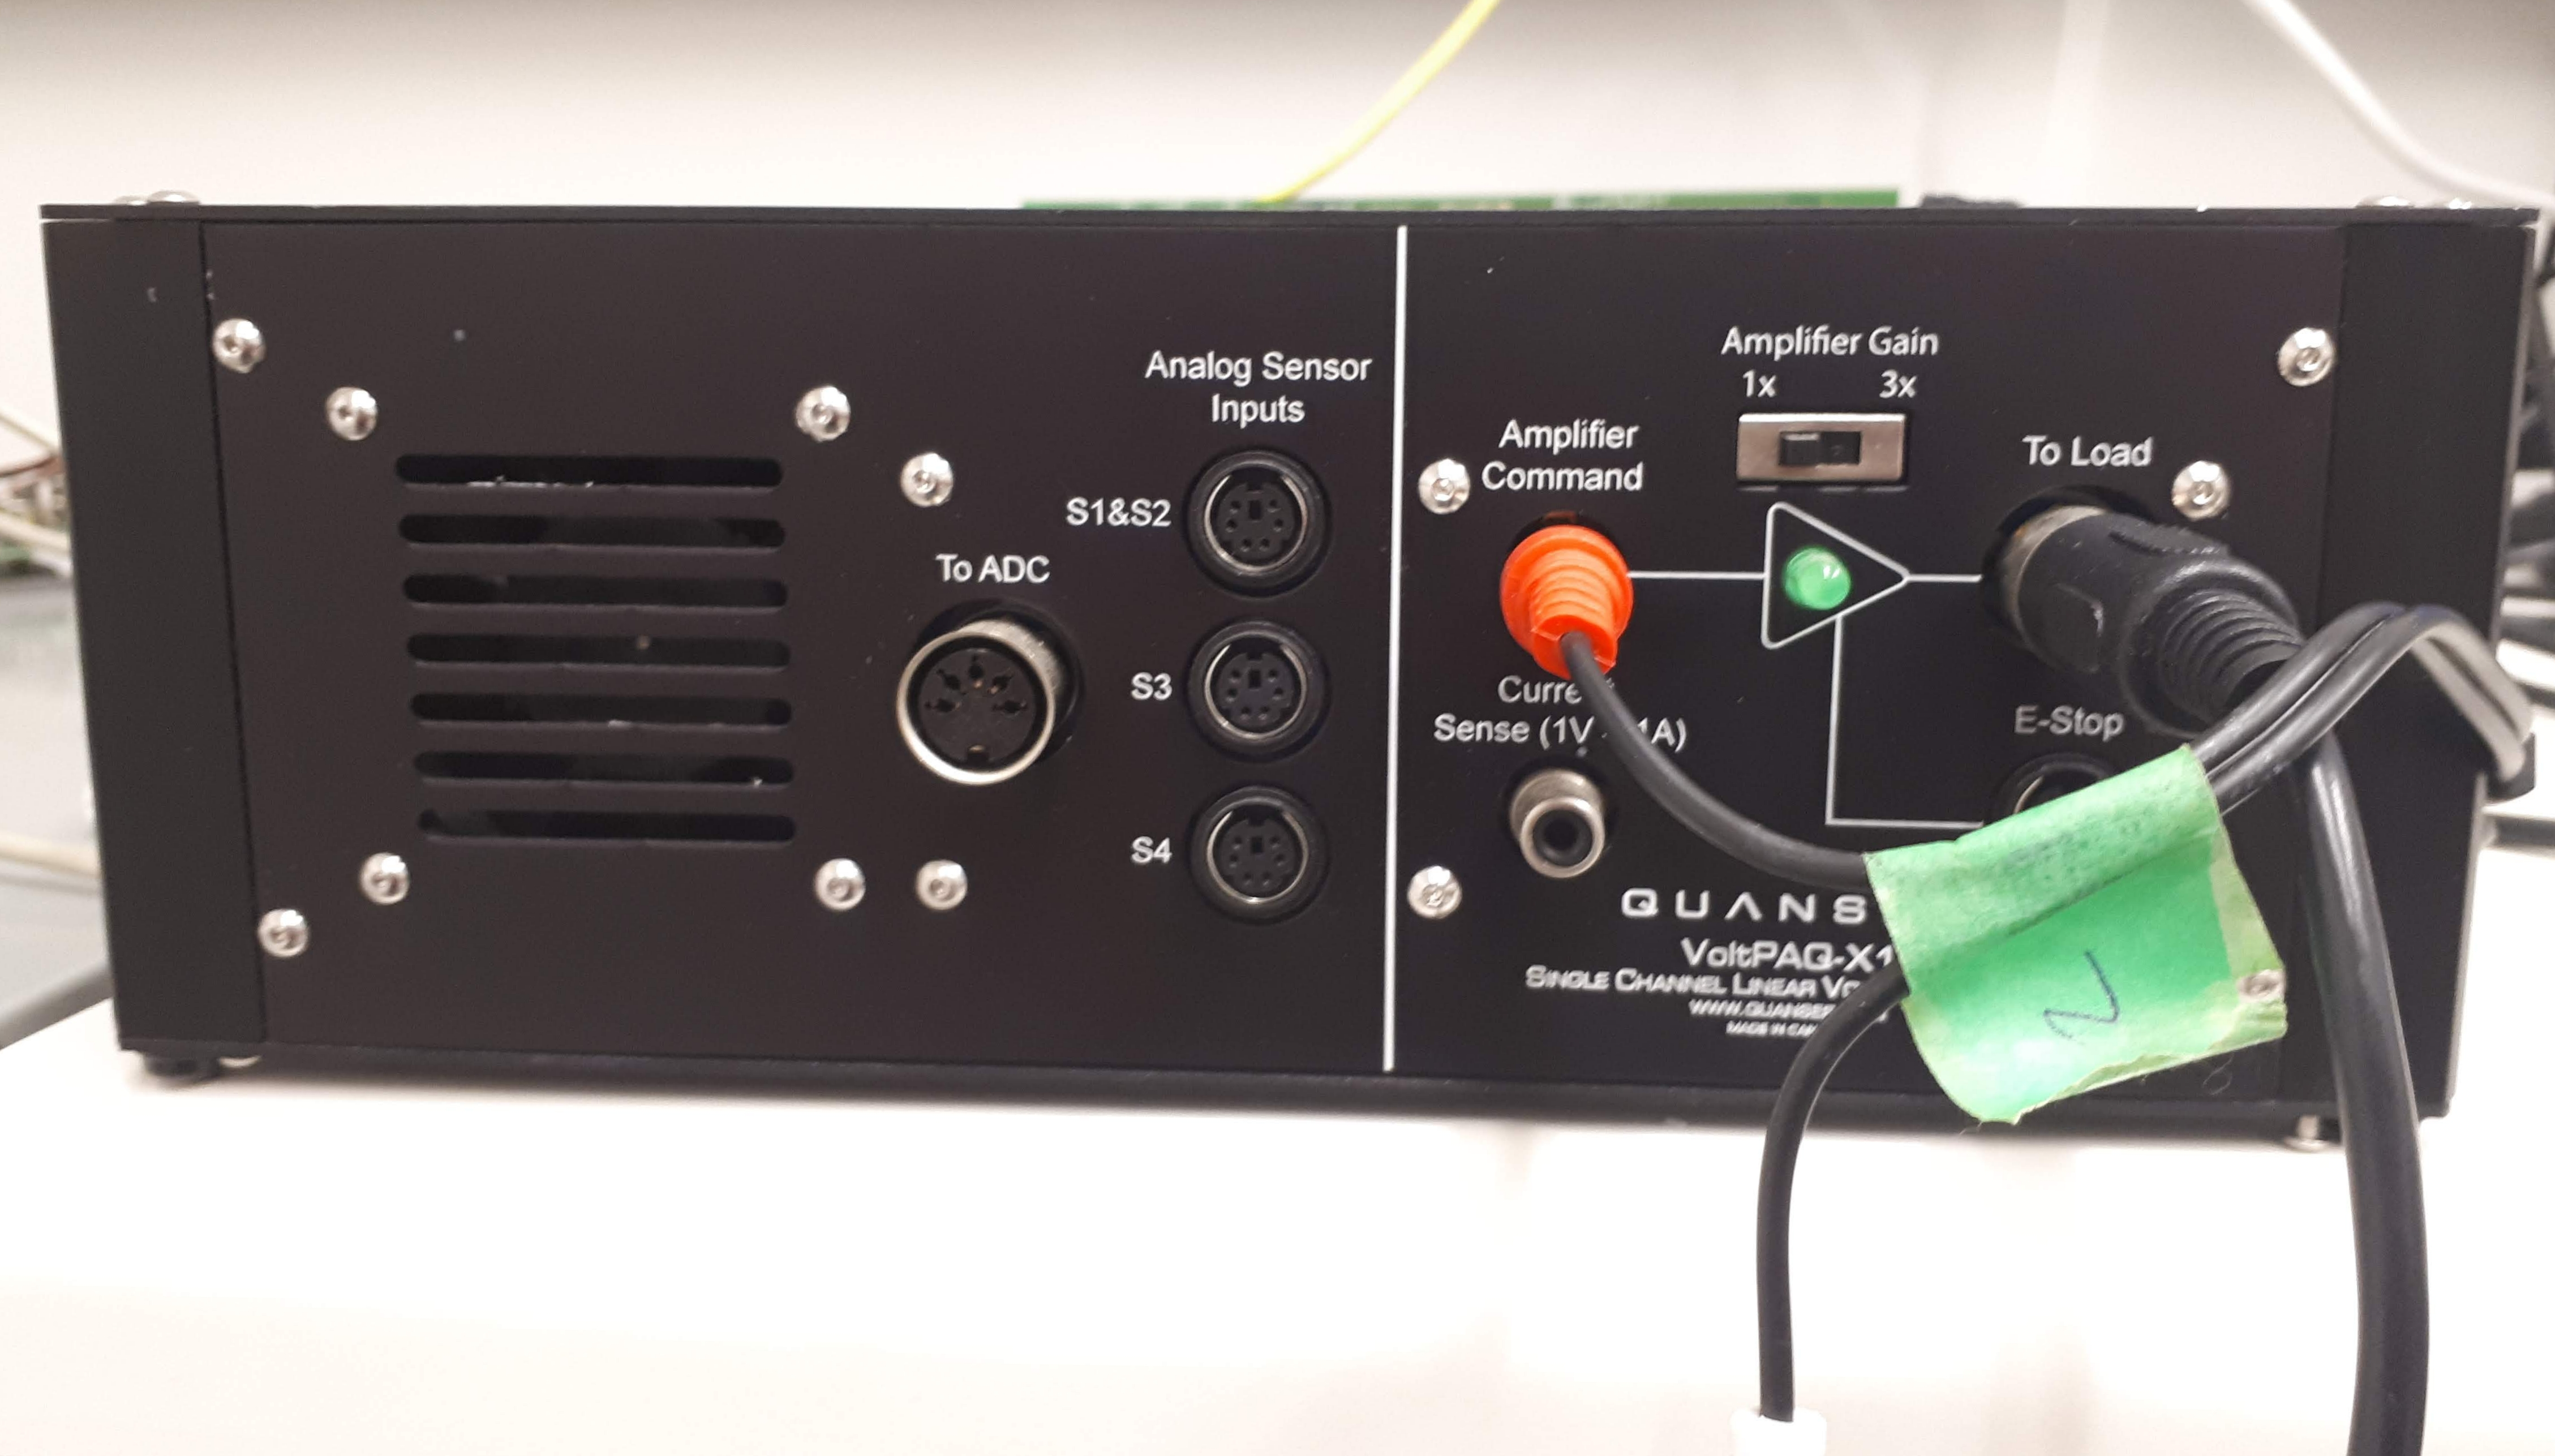
\includegraphics[scale=0.07]{img/amp.jpg}
\caption{The configuration of the VoltPAQ-X1 power amplifier for this setup}
\label{fig:amp}
\end{figure}

The pendulum base is anchored to the base plate with a clamp (temporary), and allows the rotary arm to sweep an angle of $\approx 90^{\circ}$

\begin{figure}[H]
\centering
\begin{subfigure}[b]{.4\textwidth}
    \centering
    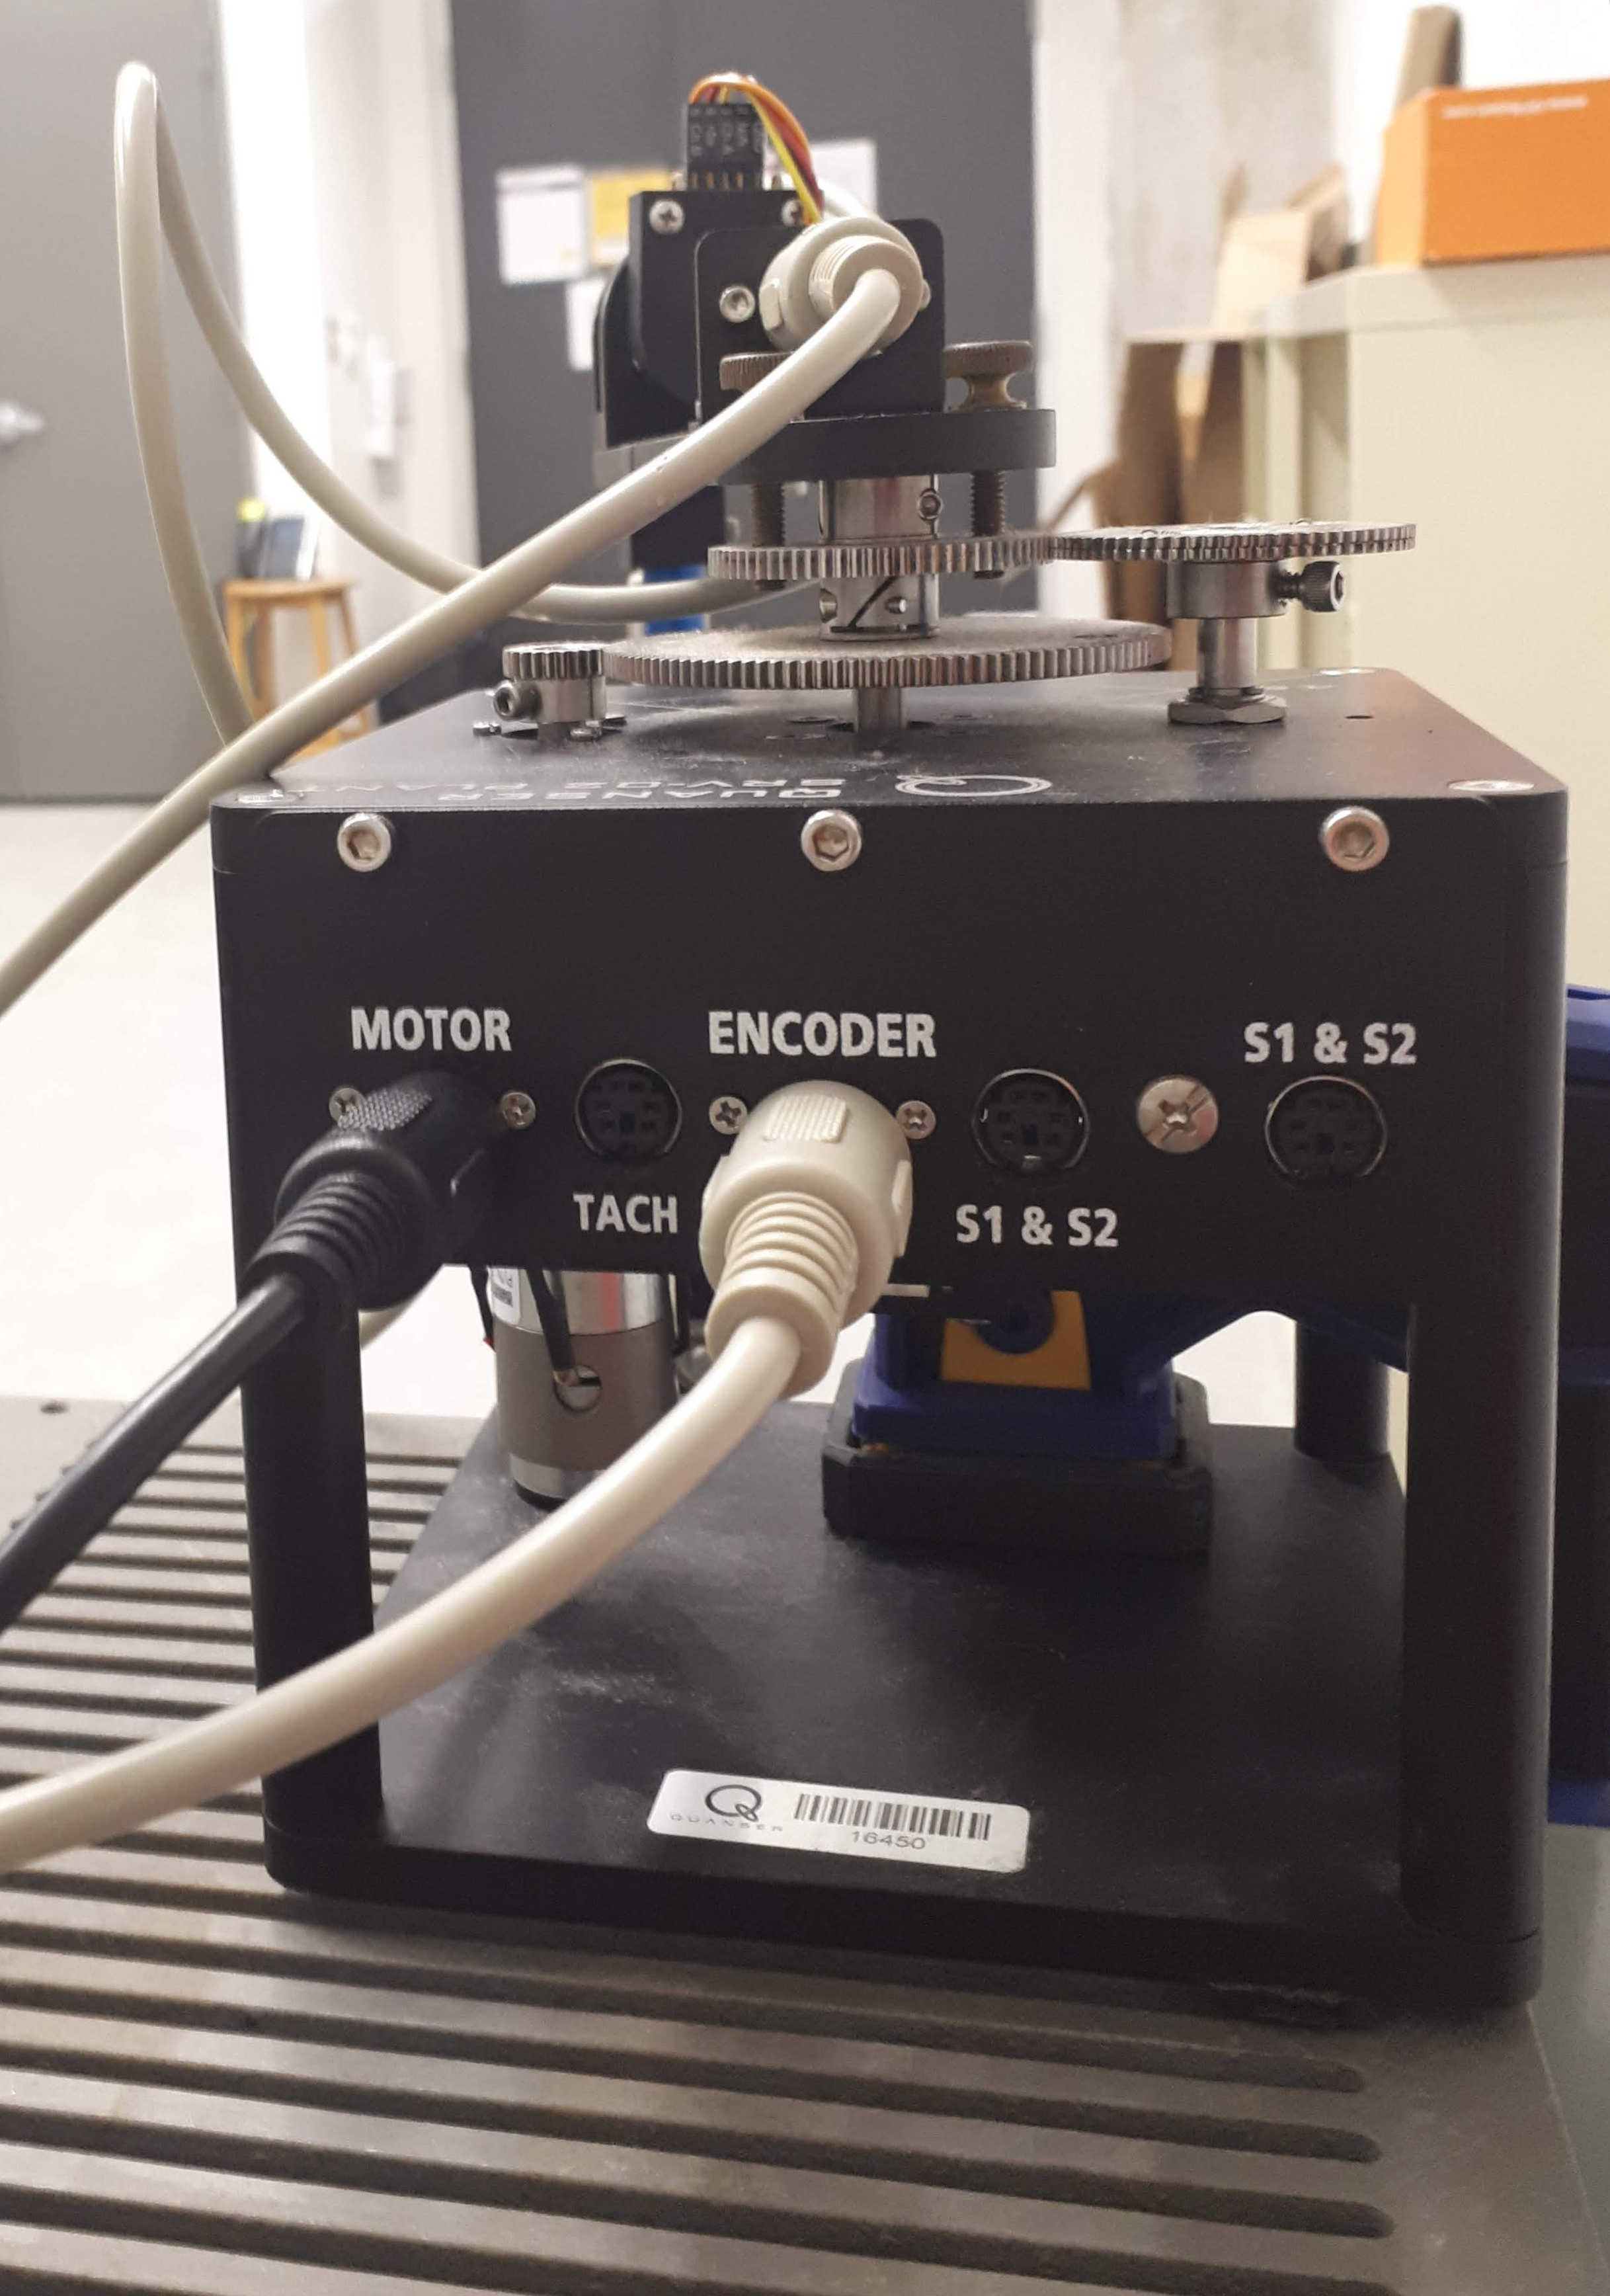
\includegraphics[width=0.7\linewidth]{img/srv02.jpg}
    \caption{The back of the SRV02 module, which is anchored to the base plate}
\end{subfigure}
%
\begin{subfigure}[b]{.45\textwidth}
    \centering
    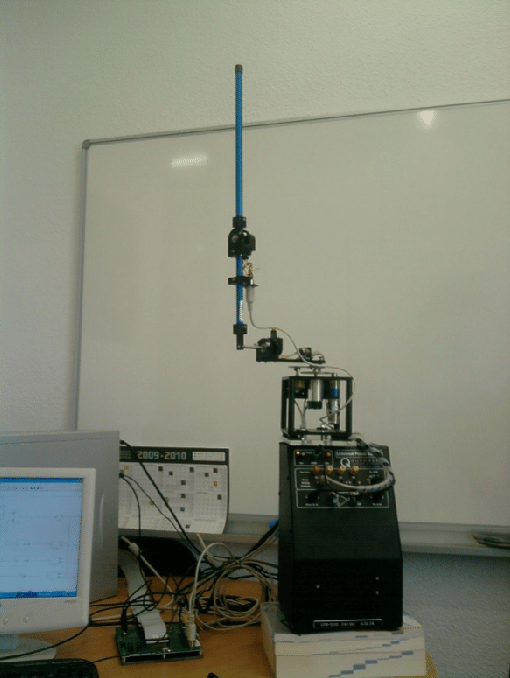
\includegraphics[width=0.7\linewidth]{img/base_alt.png}
    \caption{Potential setup to experiment with swing-up motions (minus the phonebooks)}
\end{subfigure}

\caption{The base module configuration}
\label{fig:srv}
\end{figure}

Care should be taken when manipulating the pendulum as it may hit the station on its way down when it is no longer actuated. While this basic setup is fine to run some preliminary tests for high-high balancing, it is probably not suited for swing-up experiments, as the swinging pendulums will likely hit the base during this process. An alternate design for the base is thus needed carrying forward. One option would be to elevate the SRV02 base high enough so that the swinging trajectory of both pendula remain unobstructed.

\subsection{Simulink and QUARC setup}

These setup notes are compiled from the content of previous handover documents and from the most recent installation of the system. The relevant workstation information is given below:

\begin{itemize}
    \item username: *****
    \item password: *****
    \item hostname (dhcp): *****
\end{itemize}

The current Quarc install (Quarc 2.6.1) should be working on Windows 10 with MATLAB 2017 using the Microsoft Visual C++ 2017 Family compiler. If the compiler has not been configured on MATLAB, the simulation will not be able to build:

\begin{figure}[H]
\centering
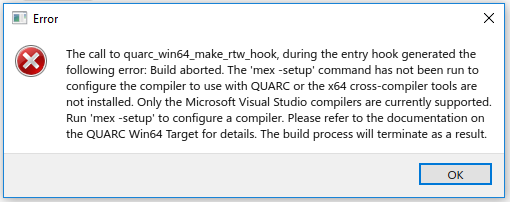
\includegraphics[width=\linewidth]{img/error.png}
\label{fig:error}
\end{figure}

Ensure that the target has been set to Win64 (\textit{quarc\_win64.tlc}) in the configuration parameters.

\begin{figure}[H]
\centering
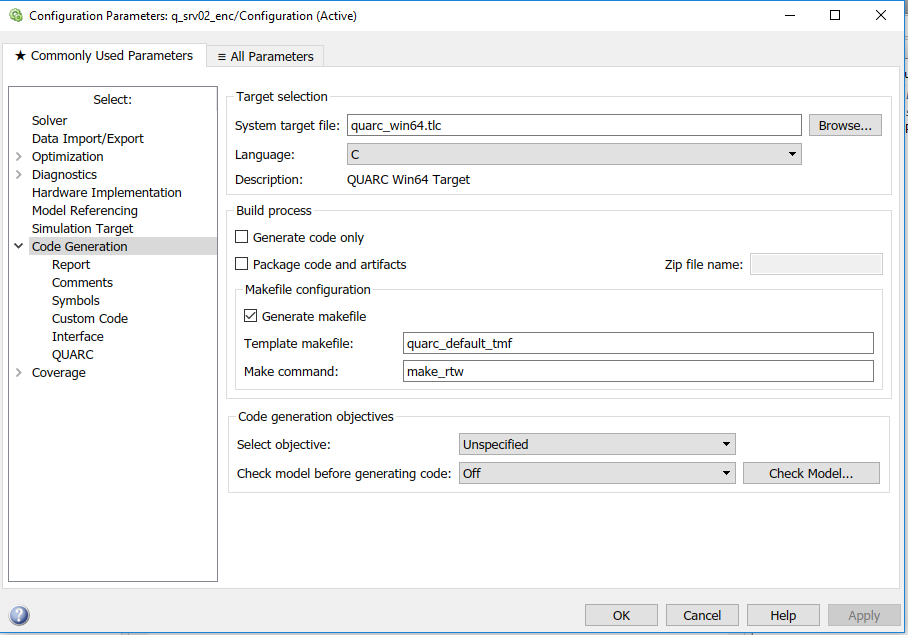
\includegraphics[width=\linewidth]{img/config.png}
\label{fig:error}
\end{figure}

In the simulink diagram, which will be similar to the one shown below, double-click on the orange box (and the one in the following window as well) to have access to the QUANSER Hardware-in-the-Loop (HIL) initialization. Double clicking the HIL Initialize block will bring up configurations pertaining to the rotary double pendulum, which includes the type of DAQ used as well as the number of inputs (\textit{i.e.} encoders). Ensure that the DAQ selected is Q8-USB (a picture should show the correct module) and set the configuration parameters to 'Default'; save the configuration. This is important for the subsequent build steps.

\begin{figure}[H]
\centering
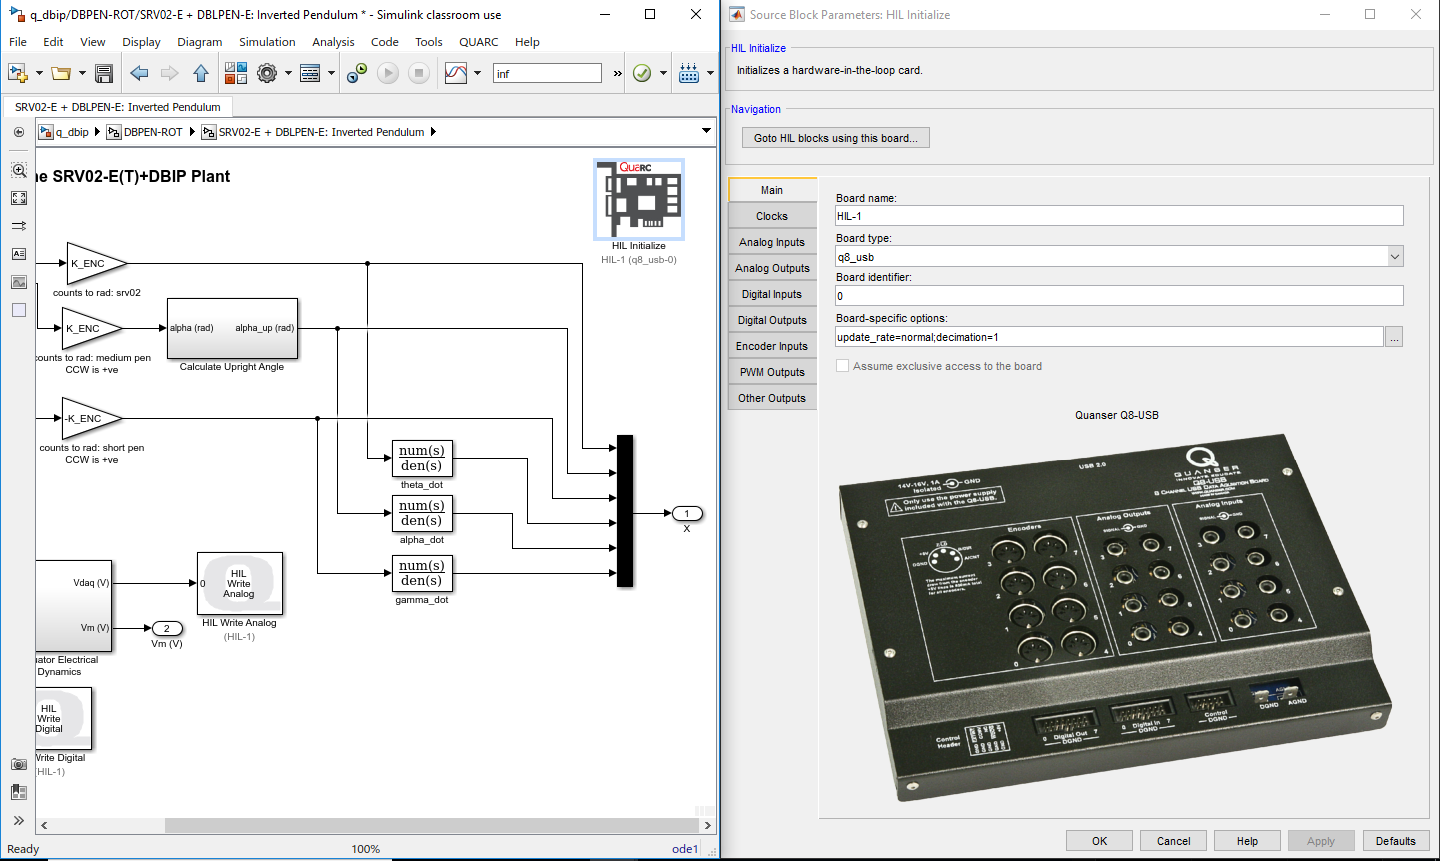
\includegraphics[width=\linewidth]{img/q8_usb.PNG}
\caption{The DAQ specified in the hardware interface needs to match the hardware}
\label{fig:simulink}
\end{figure}

The following steps describe how to run a Simulink file:

\begin{enumerate}
    \item Build the Simulink file, under QUARC>Build. This can take a few moments, you can see when it is finished in the MATLAB command window. If this fails, there is probably something wrong with the QUARC install
    \item Connect to Target (the icon that looks like two circles with triangles point to each other in them). If this fails, check over the target in the configuration parameters (check under Tools or QUARC)
    \item Run (make sure the duration is not \textbf{inf} in the Simulink window if you don’t want it to run indefinitely)
\end{enumerate}

\begin{figure}[H]
\centering
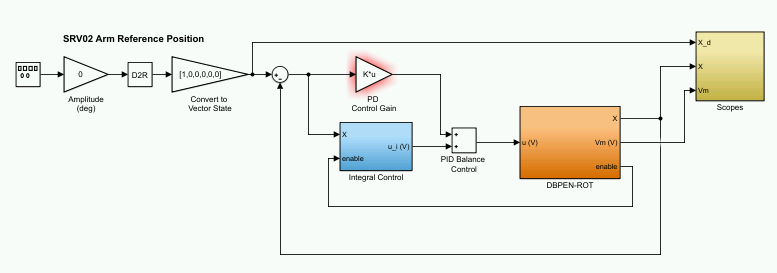
\includegraphics[width=\linewidth]{img/simulink.png}
\caption{An example of balance control system for the rotary double pendulum}
\label{fig:simulink}
\end{figure}

Make sure to catch the pendulum before hitting the stop button, as it might hit the station otherwise and potentially damage the sensors.

\section{Modelling}

\begin{figure}[H]
\centering
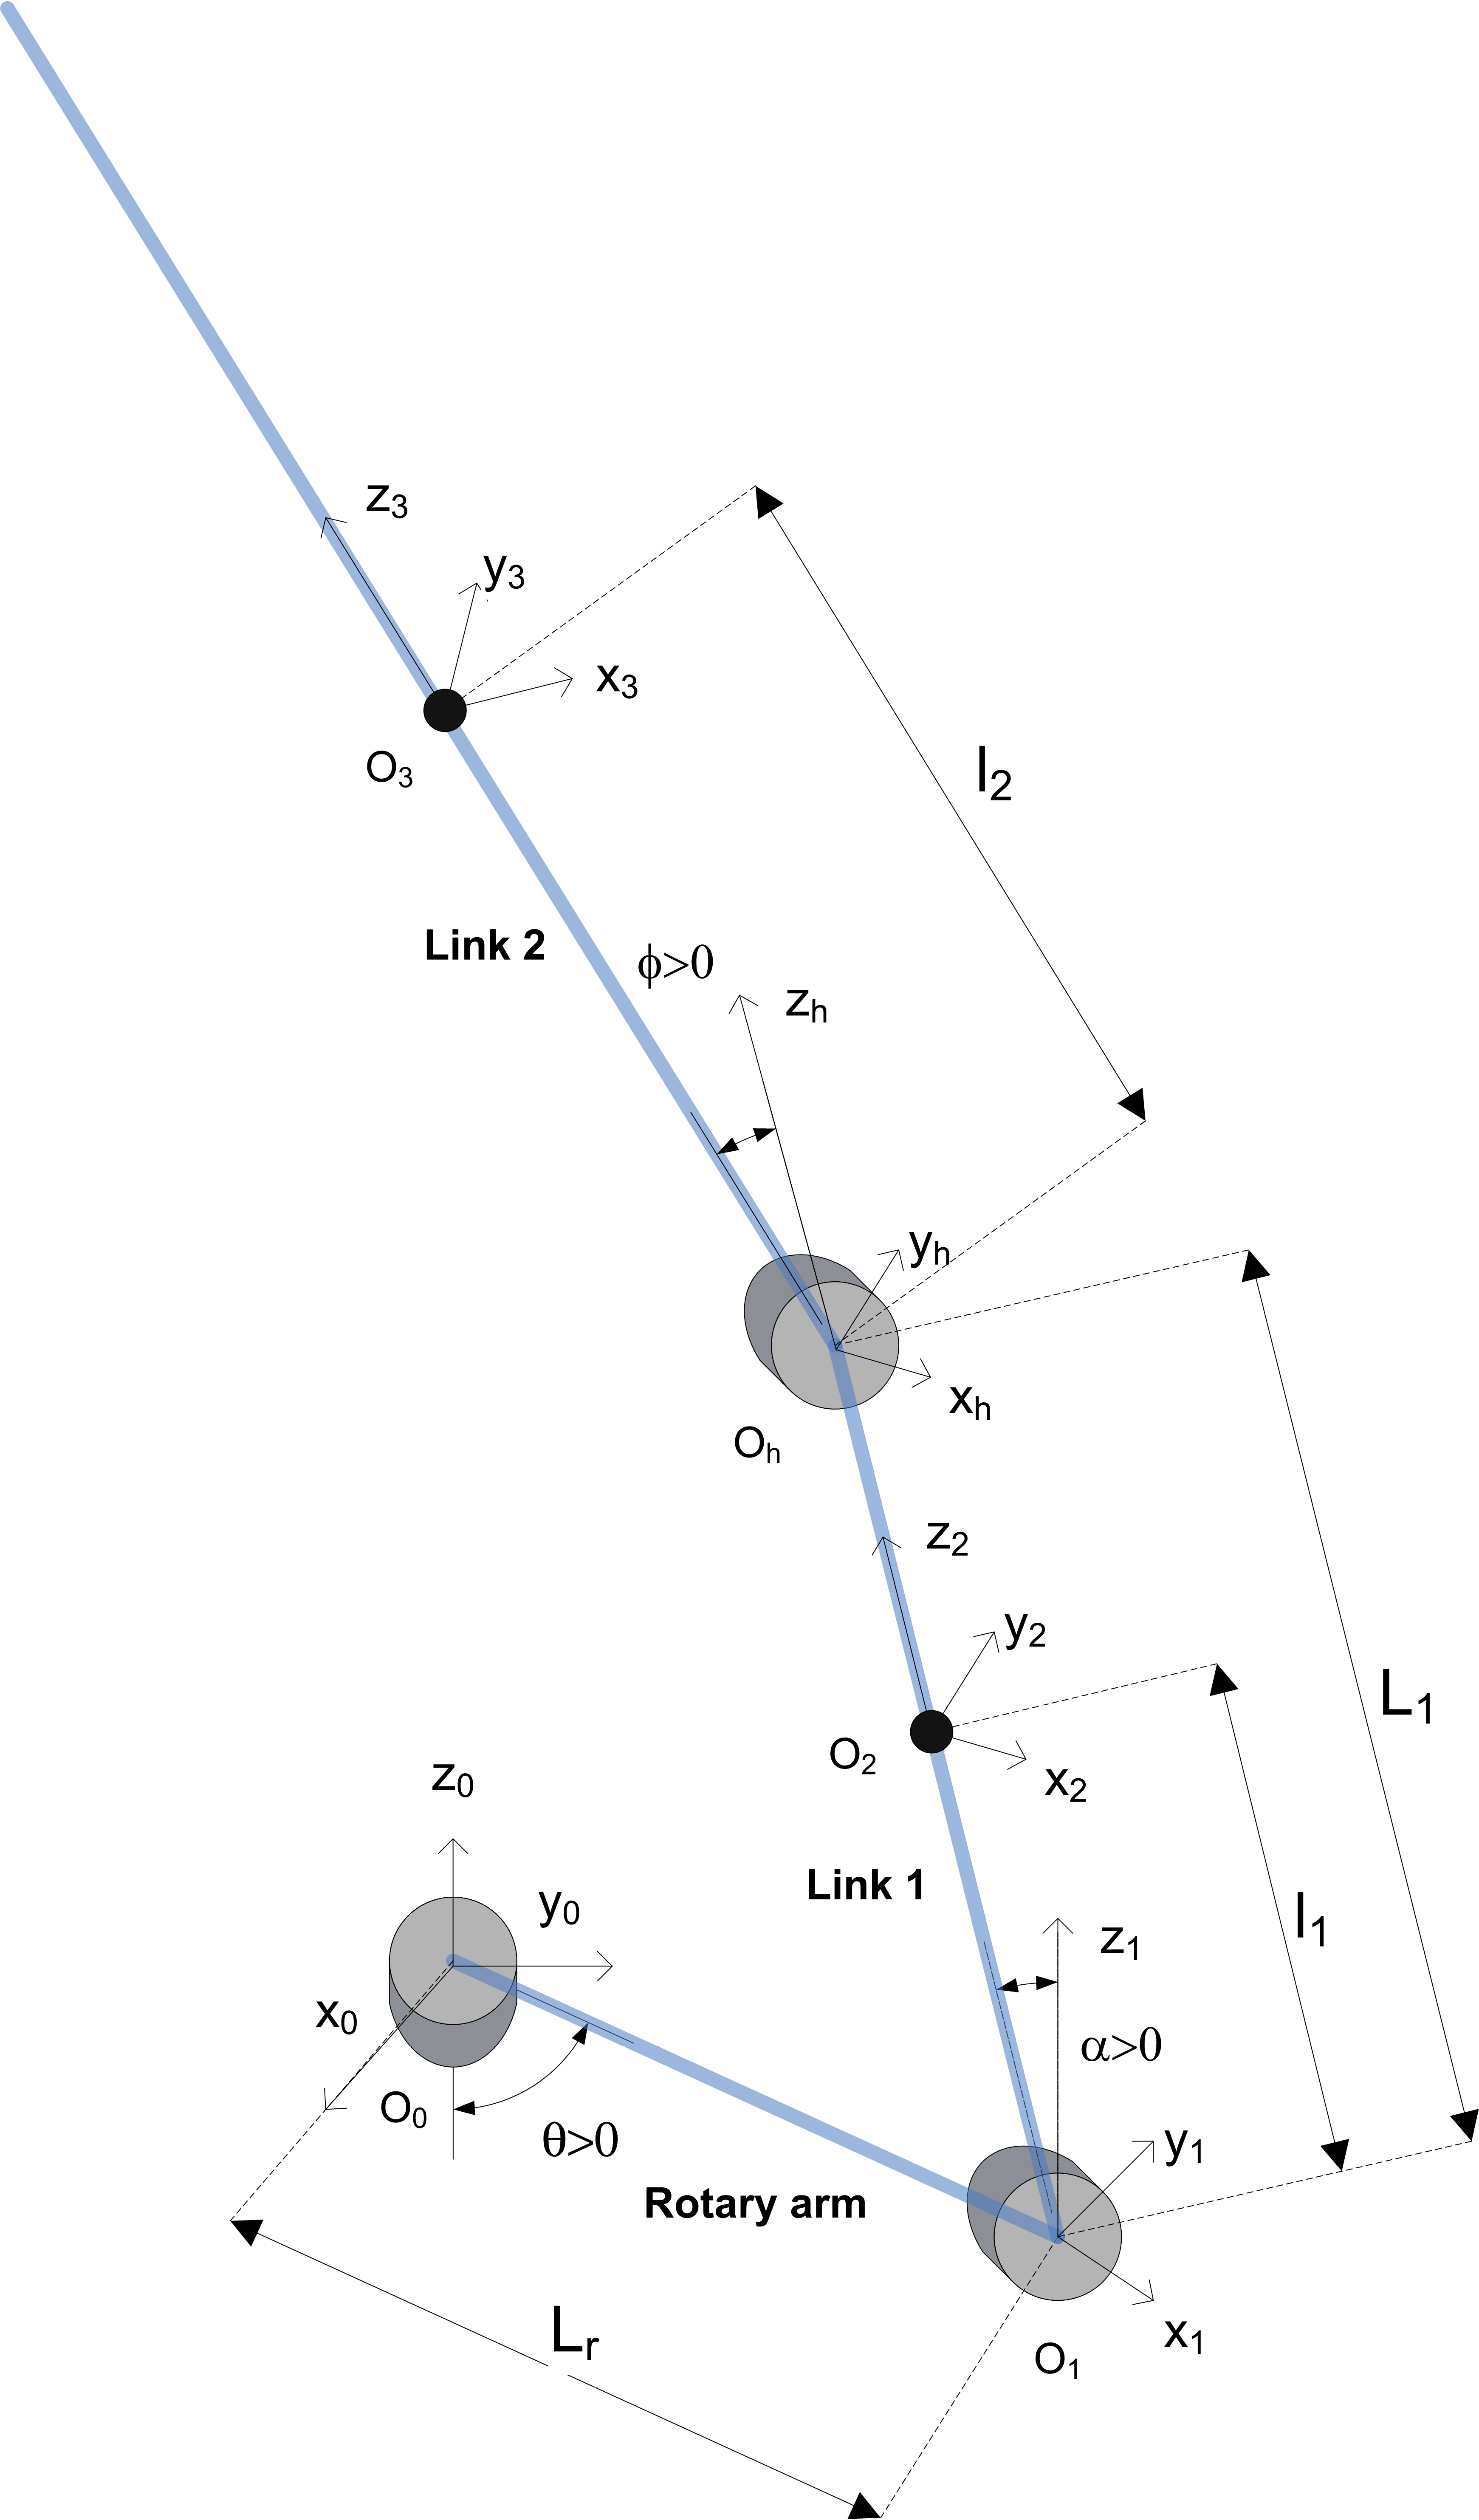
\includegraphics[scale=0.1]{img/model.png}
\label{fig:model}
\end{figure}

The 3 DOF system can be analyzed using Lagrangian dynamics by selecting the generalized coordinates to be $$q^T = \begin{bmatrix}\theta&\alpha&\phi\end{bmatrix}$$

By considering the frame $f_0$ at the origin, we can express the position of $O_1$ as $$r_1 = f_0^T \begin{bmatrix}r cos \theta\\r sin \theta\\0\end{bmatrix}$$

Similarly, by considering the frame $f_1$ at $O_1$, we can express the double pendulum arm positions as

\begin{align*}
r_2 &= f_1^T \begin{bmatrix}0\\-l_1 sin \alpha \\l_1 cos \alpha\end{bmatrix} \\
r_3 &= f_1^T \begin{bmatrix}0\\-l_1 sin \alpha -l_2 sin \phi \\l_1 cos \alpha + l_2 cos \phi \end{bmatrix}
\end{align*}

Notice that $f_1$ and $f_0$ are related by the following rotational transform

$$C_{01} = \begin{bmatrix}cos \theta&-sin \theta & 0\\sin \theta&cos \theta & 0\\0&0&1\end{bmatrix}$$

We can express all position vectors in the inertial frame $f_0$ since $r_2 = r_1 + r_2_{f_1}$ and $r_3 = r_1 + r_3_{f_1}$

\begin{align*}
r_2 &= r_1 + f_0^T C_{01} \begin{bmatrix}0\\-l_1 sin \alpha \\l_1 cos \alpha\end{bmatrix} = \begin{bmatrix}r cos \theta + l_1 sin \alpha sin \theta\\r sin \theta -l_1 sin \alpha cos \theta \\l_1 cos \alpha\end{bmatrix} \\
r_3 &= r_1 + f_0^T C_{01} \begin{bmatrix}0\\-l_1 sin \alpha -l_2 sin \phi \\l_1 cos \alpha + l_2 cos \phi \end{bmatrix} = \begin{bmatrix}r cos \theta + l_1 sin \alpha sin \theta + l_2 sin \phi sin \theta\\r sin \theta - l_1 sin \alpha cos \theta - l_2 sin \phi cos \theta \\l_1 cos \alpha + l_2 cos \phi \end{bmatrix}
\end{align*}

Next, we need to take the differentiate each position with respect to the generalized coordinates listed above. By letting $c\gamma_i = cos\gamma_i$ and $s\gamma_i = sin\gamma_i$

\begin{align*}
\Dot{r_1} &= f_0^T \begin{bmatrix}-\Dot{\theta}r s \theta \\ \Dot{\theta} r c \theta \\ 0 \end{bmatrix} \\
\Dot{r_2} &= f_0^T \begin{bmatrix}-\Dot{\theta}r s \theta + l_1 [\Dot{\theta} s \alpha c \theta + \Dot{\alpha} c \alpha s \theta]\\ \Dot{\theta} r c \theta + l_1 [\Dot{\theta} s \alpha c \theta - \Dot{\alpha} c \alpha c \theta ] \\ -l_1 \Dot{\alpha} s \alpha \end{bmatrix} \\
\Dot{r_3} &= f_0^T \begin{bmatrix}-\Dot{\theta}r s \theta + l_1 [\Dot{\theta} s \alpha c \theta + \Dot{\alpha} c \alpha s \theta] + l_2 [\Dot{\theta} s \phi c \theta + \Dot{\phi} c \phi s \theta] \\ \Dot{\theta} r c \theta + l_1 [\Dot{\theta} s \alpha c \theta - \Dot{\alpha} c \alpha c \theta ] + l_2 [\Dot{\theta} s \phi s \theta - \Dot{\phi} c \phi c \theta]\\ -l_1 \Dot{\alpha} s \alpha - l_2 \Dot{\phi} s \phi \end{bmatrix}
\end{align*}

The kinetic and potential energy of the system can then be expressed as

\begin{align*}
T &= \frac{1}{2}m_1 \Dot{r_1} \cdot \Dot{r_1} + \frac{1}{2}m_2 \Dot{r_2} \cdot \Dot{r_2} + \frac{1}{2}m_3 \Dot{r_3} \cdot \Dot{r_3} \\
V &= mg(r_2)_{f_{11}} + mg(r_3)_{f_{11}} = -2 m g l_1 cos \alpha - mg l_2 cos \phi 
\end{align*}

With $L = T - V$ defined as the lagrangian, the equations of motion of the system can be found from the following Lagrange equations

$$\frac{d}{dt}(\frac{\partial L}{\partial \Dot{q}_i}) - \frac{\partial L }{\partial q_i} = Q_i, \quad q_i \in \{\theta, \alpha, \phi\}$$

where $Q_i$ are generalized forces representing non-conservative forces acting on the system. These can be expressed in terms of the torque applied to the rotary arm (only actuated link) and the viscous damping acting on all three links.

\begin{align*}
    Q_1 &= \tau - D_r \Dot{\theta} \\
    Q_2 &= -D_{l_1} \Dot{\alpha} \\
    Q_3 &= -D_{l_2} \Dot{\phi}
\end{align*}

where $D_r$, $D_{l_1}$ and $D_{l_2}$ are damping coefficients (found in the QUANSER manuals). It is best to let MATLAB solve for the equations of motion of this system, namely $\Ddot{\theta} = f(\Dot{\theta}, \theta, t)$, $\Ddot{\alpha} = f(\Dot{\alpha}, \alpha, t)$ and $\Ddot{\phi} = f(\Dot{\phi}, \phi, t)$

\section{Future work}

Work on VHC was not started this term due to time constraints, but was introduced at a conceptual level. It should be possible to extend the current setup to achieve this in future iterations.

\pagebreak
\begin{thebibliography}{12}
\raggedright

\bibitem{quser}
Quanser Inc. Rotary Double Inverted Pendulum Experiment User Manual, 2012.

\bibitem{qlab}
Quanser Inc. Rotary Double Inverted Pendulum Experiment Laboratory Guide, 2012.

\bibitem{repo}
ljazzal. rot-double-pendulum, https://github.com/ljazzal/dynamical-systems/tree/master/rot-double-pendulum, 2019.

\end{thebibliography}

\end{document}